% !TEX TS-program = pdflatex
% !TEX encoding = UTF-8 Unicode

% This file is a template using the "beamer" package to create slides for a talk or presentation
% - Talk at a conference/colloquium.
% - Talk length is about 20min.
% - Style is ornate.

% MODIFIED by Jonathan Kew, 2008-07-06
% The header comments and encoding in this file were modified for inclusion with TeXworks.
% The content is otherwise unchanged from the original distributed with the beamer package.

\documentclass[8pt]{beamer}

% Copyright 2004 by Till Tantau <tantau@users.sourceforge.net>.
%
% In principle, this file can be redistributed and/or modified under
% the terms of the GNU Public License, version 2.
%
% However, this file is supposed to be a template to be modified
% for your own needs. For this reason, if you use this file as a
% template and not specifically distribute it as part of a another
% package/program, I grant the extra permission to freely copy and
% modify this file as you see fit and even to delete this copyright
% notice. 


\mode<presentation>
{
%\usetheme{Warsaw}
%\usetheme{Goettingen}
%\usetheme{Hannover}
\usetheme{Copenhagen}
%//FK - Ici on s'amuse avec les couleurs, ça fait mal
  % or ...
%\setbeamercolor{background canvas}{bg=red!10}
%\usecolortheme{whale}
\usecolortheme{seahorse}
%\setbeamercolor{father}{fg=red}
%\setbeamercolor{mother}{bg=green}
%\setbeamercolor{child}{parent={father,mother}}
%\begin{beamercolorbox}{child}
%Terrible red on green text.
%\end{beamercolorbox}
%\setbeamercolor{father}{fg=blue}
%\begin{beamercolorbox}{child}
%Now terrible blue on green text, since parent was changed.
%\end{beamercolorbox}
%\setbeamercolor{grandfather}{fg=red}
%\setbeamercolor{grandmother}{bg=white}
%\setbeamercolor{father}{parent={grandfather,grandmother}}
%\setbeamercolor{mother}{fg=black}
%{
%\usebeamercolor{father}\usebeamercolor{mother}
%% Defines father.fg and mother.fg globally
%}
%\setbeamercolor{my color A}{fg=father.fg!50!mother.fg}
%\setbeamercolor{my color B}{use={father,mother},fg=father.fg!50!mother.fg}
%{\usebeamercolor[fg]{my color A} dark red text}
%{\usebeamercolor[fg]{my color B} also dark red text}
%\setbeamercolor{grandfather}{fg=green}
%{\usebeamercolor[fg]{my color A} still dark red text}
%{\usebeamercolor[fg]{my color B} now dark green text}
\definecolor{UBCblue}{rgb}{0.04706, 0.13725, 0.26667} % UBC Blue (primary)

\usecolortheme[named=UBCblue]{structure}
%//FK - Ici on arrete de s'amuser avec les couleurs, ça fait trop mal

  \setbeamercovered{transparent}
  % or whatever (possibly just delete it)
}


\usepackage[english]{babel}
% or whatever
\usepackage{multicol}
\usepackage[utf8]{inputenc}
% or whatever
\usepackage{longtable}
\usepackage{times}
\usepackage[T1]{fontenc}
\usepackage{pdfpages}
\usepackage{hyperref}
\usepackage{comment}
\usepackage{textpos}
% Or whatever. Note that the encoding and the font should match. If T1
% does not look nice, try deleting the line with the fontenc.

%\getenv[\RES]{RES}\show\RES


\title[Personal introduction] % (optional, use only with long paper titles)
{Architecture And Design}

\subtitle
{Information technology}

\author[Frederic Kerdraon] % (optional, use only with lots of authors)
%{F.~Frederic Kerdraon\inst{1}}%\and S.~Another\inst{2}}
{F.~Kerdraon\inst{1}}%\and S.~Another\inst{2}}
% - Give the names in the same order as the appear in the paper.
% - Use the \inst{?} command only if the authors have different
%   affiliation.

\institute[University of theoretical physics] % (optional, but mostly needed)
{
  \inst{1}%
  Department of Computer Science\\
  Global Business Analyst  
%  \and
%  \inst{2}%
%  Department of Theoretical Philosophy\\
%  University of Elsewhere}
% - Use the \inst command only if there are several affiliations.
% - Keep it simple, no one is interested in your street address.
}

\date[CFP 2016] % (optional, should be abbreviation of conference name)
{Conference on the Information Technology}
% - Either use conference name or its abbreviation.
% - Not really informative to the audience, more for people (including
%   yourself) who are reading the slides online

\subject{Theoretical Computer Science}
% This is only inserted into the PDF information catalog. Can be left
% out. 


\excludecomment{mysection}

% If you have a file called "university-logo-filename.xxx", where xxx
% is a graphic format that can be processed by latex or pdflatex,
% resp., then you can add a logo as follows:

 \pgfdeclareimage[height=0.7cm]{Logo}{Logo.png}
 \logo{\pgfuseimage{Logo}}



% Delete this, if you do not want the table of contents to pop up at
% the beginning of each subsection:
%//FK - Removed because I don't need this
%\AtBeginSubsection[]
%{
%  \begin{frame}<beamer>{Personal introduction}
%    %\tableofcontents[Help, Automate]
%  \end{frame}
%}


% If you wish to uncover everything in a step-wise fashion, uncomment
% the following command: 

%\beamerdefaultoverlayspecification{<+->}



\begin{document}

\begin{frame}
  \titlepage
\begin{textblock*}{0cm}(0.01cm,-7.4cm)
   %\rule{1cm}{1cm}\includegraphics[scale=0.3]{Logo.png}
   \includegraphics[scale=0.2]{Logo.png}
\end{textblock*}
\footnote{
\tiny{Resume :\url{Resume.pdf} }
}
\end{frame}


\begin{frame}{Table of contents}
\begin{multicols}{2}
  \tableofcontents
  % You might wish to add the option [pausesections]
\end{multicols}
\end{frame}


% Structuring a talk is a difficult task and the following structure
% may not be suitable. Here are some rules that apply for this
% solution: 

% - Exactly two or three sections (other than the summary).
% - At *most* three subsections per section.
% - Talk about 30s to 2min per frame. So there should be between about
%   15 and 30 frames, all told.

% - A conference audience is likely to know very little of what you
%   are going to talk about. So *simplify*!
% - In a 20min talk, getting the main ideas across is hard
%   enough. Leave out details, even if it means being less precise than
%   you think necessary.
% - If you omit details that are vital to the proof/implementation,
%   just say so once. Everybody will be happy with that.

\section{Project management}

\begin{frame}{Project management}
  % - A title should summarize the slide in an understandable fashion
  %   for anyone how does not follow everything on the slide itself.
\begin{multicols}{2}
[
]
 \begin{itemize}
  \item
   People 
  \item
   Methodologies 
  \item
   Deliverables 
  \item
   Meetings 
  \item
   Reporting 
  \item
   Communication 
 \end{itemize}
%\includegraphics[scale=0.3]{/home/frederickerdraon/Documents/images/MilkDrop.png}
\includegraphics[scale=0.15]{shutterstock.jpg}
\end{multicols}
\footnote{
\tiny{Project :\url{Project.pdf} }
}
%\footnote{
%\tiny{John Dryden : All human things are subject to decay. And when fate summons, Monarchs must obey.}
%}

\end{frame}

\subsection{Structure}

\begin{frame}{People}
\begin{multicols}{2}
[
]
 \begin{itemize}
  \item
    Why it's important 
  \item
    Different ways to communicate 
  \item
    How you know it worked 
  \item
    Why it's important to formalize 
 \end{itemize}
\tiny{Website,Blog,Email,Teamviewer,Youtube,Social networks(LinkedIn, Facebook, Twitter,etc),Chats(Slack),Intranet,Formal letters.}
\includegraphics[scale=0.15]{monday-morning.png}
\end{multicols}
\footnote{
\tiny{People :\url{Perso.pdf} }
}
\end{frame}

\begin{frame}{Methodologies}
\begin{multicols}{2}
[]
 \begin{itemize}
  \item
    Why it's important
  \item
    Different ways to communicate
  \item
    How you know it worked
  \item
    Why it's important to formalize
 \end{itemize}
\includegraphics[scale=0.15]{Methodology.jpg}
\end{multicols}
\footnote{
\href[Methodology]{http://localhost/mediawiki-1.23.9/index.php/Project\_management\#Meetings}{Methodology wiki}
}
\end{frame}

\begin{frame}{Deliverables}
\begin{multicols}{2}
[
]
 \begin{itemize}
  \item
    Why it's important
  \item
    Different ways to communicate
  \item
    How you know it worked
  \item
    Why it's important to formalize
 \end{itemize}
\includegraphics[scale=0.15]{Blocks.png}
\end{multicols}
\footnote{
\href[Deliverables]{http://localhost/mediawiki-1.23.9/index.php/Project\_management\#Meetings}{Deliverables wiki}
}
\end{frame}


\begin{frame}{Meetings}
\begin{multicols}{2}
[
]
 \begin{itemize}
  \item
    Steering comittee 
  \item
    Cross projects meeting 
  \item
    Team meeting 
 \end{itemize}
\includegraphics[scale=0.05]{TeamMeetings.jpg}
\end{multicols}
\footnote{
\href[Meetings]{http://localhost/mediawiki-1.23.9/index.php/Project\_management\#Meetings}{Meetings wiki}
}
\end{frame}

\begin{frame}{Reporting}
\begin{multicols}{2}
[
]
 \begin{itemize}
  \item
    Steering comittee 
  \item
    Cross projects meeting 
  \item
    Team meeting 
 \end{itemize}
\includegraphics[scale=0.05]{TeamMeetings.jpg}
\end{multicols}
\footnote{
\href[Reporting]{http://localhost/mediawiki-1.23.9/index.php/Project\_management\#Meetings}{Reporting wiki}
}
\end{frame}

\begin{frame}{Communication}
\begin{multicols}{2}
[
]
 \begin{itemize}
  \item
    Team meeting 
  \item
    Cross projects meeting 
  \item
    Monthly stake holders meeting 
 \end{itemize}
\includegraphics[scale=0.05]{TeamMeetings.jpg}
\end{multicols}
\footnote{
\href[Communication]{http://localhost/mediawiki-1.23.9/index.php/Project\_management\#Meetings}{Communication wiki}
}
\end{frame}
%\subsection{Methodologies}

%\specialcomment{mysection}{\begingroup\color{gray}}{\endgroup}A

%\begin{comment}

%\begin{frame}{Methodologies}
%  You can create overlays\dots
%  \begin{itemize}
%  \item using the \texttt{pause} command:
%    \begin{itemize}
%    \item
%      First item.
%      \pause
%    \item    
%      Second item.
%    \end{itemize}
%  \item
%    using overlay specifications:
%    \begin{itemize}
%    \item<3->
%      First item.
%    \item<4->
%      Second item.
%    \end{itemize}
%  \item
%    using the general \texttt{uncover} command:
%    \begin{itemize}
%      \uncover<5->{\item
%        First item.}
%      \uncover<6->{\item
%        Second item.}
%    \end{itemize}
%  \end{itemize}
%\end{frame}

%\end{comment}

\subsection{Deliverables}

\begin{frame}{Project inception}
Owner : Project manager\\
Contributors : Stake holders, Business analysts\\
 \begin{itemize}
  \item
- What is the purpose (Returns, Criticality)?
  \item
- How are we supposed to do that? 
  \item
- Who are the sponsors/resources for this project?
  \item
- When is it expected to be delivered?
  \item
- What are we supposed to deliver?
 \end{itemize}
\footnote{
\footnotesize{
\tiny{Project initiation :\url{Inception.pdf} }}
}
\end{frame}

\begin{frame}{Feasability study}
Owner : Project manager\\
Contributors : Stake holders, Business analysts\\
 \begin{itemize}
  \item
- Who is doing it 
  \item
- Data requirements 
  \item
- Process requirements 
  \item
- Resources needed 
  \item
- Sign off 
 \end{itemize}
\footnote{
\footnotesize{
\tiny{Feasability :\url{Feasability.pdf} }}
}
\end{frame}

\begin{frame}{Clearchoice}
Owner : Project manager\\
Contributors : Stake holders, Business analysts\\
 \begin{itemize}
  \item
%    \texttt{MySql}
- Choice 1
  \item
%    \texttt{MySql}
- Choice 2
  \item
- Do nothing
  \item
- Sign off 
 \end{itemize}
\footnote{
\footnotesize{
\tiny{Clearchoice :\url{Clearchoice.pdf} }}
}
\footnote{
\tiny{Nietzsche : « Le mensonge le plus courant est celui que l'on se fait à soi-même ; mentir aux autres est plutôt l'exception. »}
}
\end{frame}

\begin{frame}{Proof of concept}
Owner : Project manager\\
Contributors : Stake holders, Business analysts\\
 \begin{itemize}
  \item
%    \texttt{MySql}
- Technology 1
  \item
%    \texttt{MySql}
- Technology 2
  \item
- Sign off 
 \end{itemize}
\footnote{
\footnotesize{
\tiny{Proof of concept :\url{Proof.pdf} }}
}
\end{frame}

\begin{frame}{Specifications}
Owner : Business analyst\\
Contributors : Business analysts\\
 \begin{itemize}
  \item
- User interface
  \item
- Business workflow
  \item
- Business component
  \item
- Input data
  \item
- Output data
  \item
- Sign off 
 \end{itemize}
\footnote{
\footnotesize{
\tiny{Specifications :\url{Specifications.pdf} }}
}
\end{frame}

\begin{frame}{Internal design}
Owner : Business analyst\\
Contributors : Business analysts\\
- 
\footnote{
\footnotesize{
\tiny{Internal design :\url{Internal.pdf} }}
}
\end{frame}

\begin{frame}{External design}
Owner : Business analyst\\
Contributors : Business analysts\\
\footnote{
\footnotesize{
\tiny{External design :\url{External.pdf} }}
}
\end{frame}

\begin{frame}{Test documentation}
Owner : Business analyst\\
Contributors : Business analysts\\
\footnote{
\footnotesize{
\tiny{Test documentation :\url{Test.pdf} }}
}
\end{frame}

\begin{frame}{User Manual}
Owner : Business analyst\\
Contributors : Business analysts\\
\footnote{
\footnotesize{
\tiny{User Manual :\url{UserManual.pdf} }}
}
\end{frame}

\begin{frame}{Production release}
Owner : Project manager\\
Contributors : Business analysts\\
\footnote{
\footnotesize{
\tiny{Production release :\url{Release.pdf} }}
}
\end{frame}

\subsection{Meetings}

\begin{frame}{Daily team meeting}
\end{frame}
\begin{frame}{Weekly managers meeting}
\end{frame}
\begin{frame}{Monthly stake holders meeting}
\footnote{
%\footnotesize{
\tiny{Project inception :\url{Inception.pdf} }}
%}
\footnote{
\href[Meetings]{http://localhost/mediawiki-1.23.9/index.php/Project\_management\#Meetings}{Meeting wiki}
}
\end{frame}

\subsection{Reporting}

\begin{frame}{Steering comittee}
\begin{multicols}{2}
[
]
\begin{itemize}
  \item
- Budget
  \item
- Planning \& milestones
  \item
- Risks
  \item
- Aggregated tasks
  \item
- People 
\end{itemize}
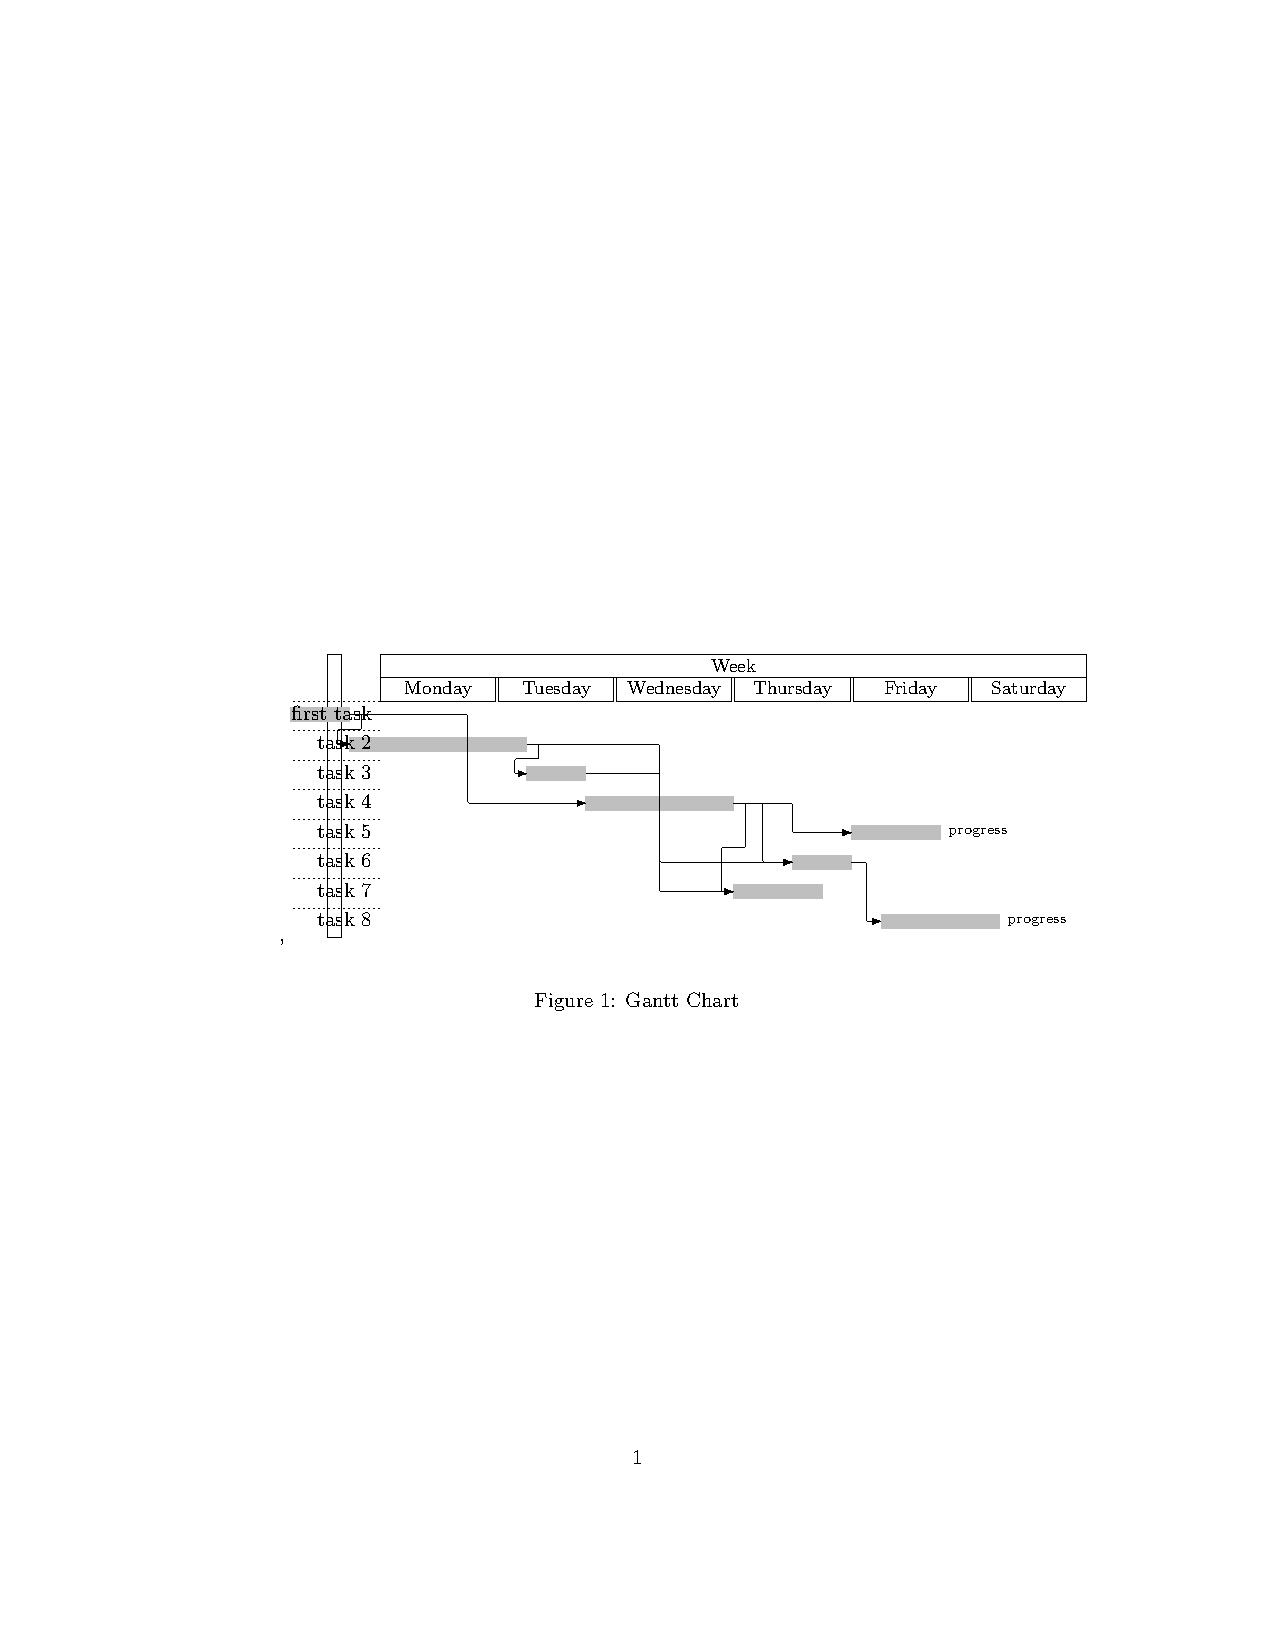
\includegraphics[scale=0.30]{Gantt.png}
%\documentclass[landscape]{article}
\usepackage{pgfgantt}
\usepackage[landscape]{geometry}

\begin{document}

\begin{figure}[ftbp]
\begin{center}

\definecolor{RoyalBlue}{RGB}{153,204,254}
 
\begin{ganttchart}[y unit title=0.4cm,y unit chart=0.5cm,
vgrid,hgrid,
title label anchor/.style={below=-1.6ex},
title/.append style={draw=none, fill=RoyalBlue!50!black},
%title left shift=.05,
title left shift=0,
%title right shift=-.05,
title right shift=0,
title height=1,
%bar/.style={fill=gray!50},
bar/.style={fill=RoyalBlue},
bar incomplete/.style={fill=RoyalBlue},
progress label text={progressing},
bar height=0.3,
group right shift=.4,
group top shift=.6,
group height=.3,
group/.append style={draw=black, fill=green!50},
milestone/.append style={fill=black, rounded corners=3pt},
bar/.append style={fill=red, rounded corners=3pt}
%group peaks={0}{0}{.2}
%]{0}{2},
%vrule/.style={very thick, blue}
%vrule label font=\bfseries
]{0}{23},

%labels

\gantttitle{Week}{24} \\
\gantttitle{Monday}{4} 
\gantttitle{Tuesday}{4} 
\gantttitle{Wednesday}{4} 
\gantttitle{Thursday}{4} 
\gantttitle{Friday}{4} 
\gantttitle{Saturday}{4} \\

%tasks
\ganttgroup{Group 1}{1}{10} \\
\ganttbar[progress=50]{Inception}{1}{2} \\
\ganttbar{Feasability study}{3}{8} \\
\ganttbar{Clearchoice}{9}{10} \\
\ganttbar{Proof of concept}{11}{15} \\
\ganttbar[progress=33]{Specifications}{20}{22} \\
\ganttbar{Internal design}{18}{19} \\
\ganttbar{External design}{16}{18} \\
\ganttbar[progress=0]{Release}{21}{23}\\
\ganttbar[progress=0]{task 8}{2}{21}\\
\ganttbar[progress=0]{task 8}{2}{21}\\
\ganttbar[progress=0]{task 8}{2}{21}\\
\ganttbar[progress=0]{task 8}{2}{21}\\
\ganttbar[progress=0]{task 8}{2}{21}\\

%\ganttvrule[
%vrule/.append style={red, thin},
%vrule offset=.2
%]{day z}{6}

%milestones
\ganttmilestone{Milestone 1}{11}

%relations

\ganttlink{elem0}{elem1}
\ganttlink{elem0}{elem3}
\ganttlink{elem1}{elem2}
\ganttlink{elem3}{elem4}
\ganttlink{elem1}{elem5}
\ganttlink{elem3}{elem5}
\ganttlink{elem2}{elem6}
\ganttlink{elem3}{elem6}
\ganttlink{elem5}{elem7}
%\ganttlink{elem8}{elem9}

\end{ganttchart}

\end{center}

\caption{Gantt Chart}

\end{figure}

\end{document}

\end{multicols}
\footnote{
\tiny{Management summary :\url{Management.pdf} }
}
\end{frame}

\begin{frame}{Cross projects reports}
  \begin{itemize}
  \item
- Infrastructure
  \item
- Tools
  \end{itemize}
\footnote{
\tiny{Cross project report :\url{CrossProjectReport.pdf} }
}
\end{frame}

\begin{frame}{Team report}
  \begin{itemize}
  \item
- Tasklist
  \item
- Burndown
  \item
- Events (Calendar)
  \end{itemize}
\footnote{
\tiny{Team report :\url{TeamReport.pdf} }
}
\end{frame}

\begin{frame}{Meeting minutes}
  \begin{itemize}
  \item
- Stake holder's meeting
  \item
- Cross project meetings
  \item
- Team meetings
  \end{itemize}
\footnote{
\tiny{Meeting minutes :\url{Meeting\_Minutes.pdf} }
}
\end{frame}

\section{Information technology}
\subsection{Infrastructure}

\begin{frame}{Infrastructure}
  \begin{itemize}
  \item
- Database 
  \item
- Hardware 
  \item
- Code review
  \item
- Change management 
  \end{itemize}
\end{frame}

\subsection{Tech documentation}

\begin{frame}{Tech documentation}
  \begin{itemize}
  \item
- Code comments
  \item
- Project documentation 
  \end{itemize}
\end{frame}

\section{Finance}
\subsection{Corporate finance}

\begin{frame}{General}
Corporate finance
  \begin{itemize}
  \item
- Management summary 
  \item
- Cash balance management 
  \item
- Assets and liabilities management 
  \end{itemize}
\footnote{
\tiny{Finance :\url{Finance.pdf} }
}
\end{frame}

\begin{frame}{Cash balance management}
Equities
  \begin{itemize}
  \item
- Stock 
  \item
- Options 
  \item
- ETFs
  \end{itemize}
\footnote{
\tiny{Cash balance :\url{Finance-Cash-Balance.pdf} }
}
\end{frame}

\begin{frame}{Asset liabilities management}
Equities
  \begin{itemize}
  \item
- Stock 
  \item
- Options 
  \item
- ETFs
  \end{itemize}
\footnote{
\tiny{ALM :\url{Finance-Assets-Liabilities.pdf} }
}
\end{frame}

\subsection{Pricing}

\begin{frame}{Pricing}
Equities
  \begin{itemize}
  \item
- Stock 
  \item
- Options 
  \item
- ETFs
  \end{itemize}
\footnote{
\tiny{Stocks :\url{Finance-Stocks.pdf} }
}
\end{frame}

\begin{frame}{Pricing}
Interest rates
  \begin{itemize}
  \item
- Vanillas 
  \item
- Options 
  \item
- Structured products 
  \end{itemize}
\end{frame}

\begin{frame}{Pricing}
Fixed income
 \begin{itemize}
  \item
- Treasury bonds 
  \item
- Burndown
  \item
- Events (Calendar)
  \end{itemize}
\end{frame}

\begin{frame}{Pricing}
Currencies
  \begin{itemize}
  \item
- Vanillas 
  \item
- Options 
  \item
- Structured products 
  \end{itemize}
\footnote{
\tiny{Foreign Exchange :\url{Finance-Currencies.pdf} }
}
\end{frame}

\begin{frame}{Pricing}
Structured investment vehicules
  \begin{itemize}
  \item
- Assets liabilities basics 
  \item
- Monte carlo simulations 
  \item
- Why it failed 
  \end{itemize}
\end{frame}

\subsection{Risk management}
\begin{frame}{Risk management}
Sensitivities
  \begin{itemize}
  \item
- Delta 
  \item
- Beta 
  \item
- Gamma 
  \end{itemize}
\end{frame}

\begin{frame}{Risk management}
Parametric Value at Risk
  \begin{itemize}
  \item
- Delta 
  \item
- Beta 
  \item
- Gamma 
  \end{itemize}
\end{frame}

\begin{frame}{Risk management}
Historical Value at Risk
  \begin{itemize}
  \item
- Delta 
  \item
- Beta 
  \item
- Gamma 
  \end{itemize}
\end{frame} 

\begin{frame}{Risk management}
Stress testing
  \begin{itemize}
  \item
- Equities 
  \item
- Interest rates 
  \item
- Fixed income 
  \end{itemize}
\end{frame} 

\section{Conclusion}

\subsection{Main Results}

\begin{frame}{Acheivements}
\end{frame}

\begin{frame}{Collaborations}
\end{frame}

\begin{frame}{Resources}
  \begin{itemize}
  \item
- Intranet
  \item
- Website
  \item
- Blog
  \item
- LinkedIn
  \end{itemize}
\end{frame}

\begin{frame}{Current projects}
  \begin{itemize}
  \item
- Artificial intelligence
  \item
- Blockchain
  \end{itemize}
\end{frame}


\subsection{Future projects}

\begin{frame}{Quantum computing}
\end{frame}

\begin{frame}{Relativity}
\end{frame}

\begin{frame}{Quantum theory}
\end{frame}



\section*{Summary}

\begin{frame}{Summary}

  % Keep the summary *very short*.
  \begin{itemize}
  \item
    The \alert{first main message} of your talk in one or two lines.
  \item
    The \alert{second main message} of your talk in one or two lines.
  \item
    Perhaps a \alert{third message}, but not more than that.
  \end{itemize}
  
  % The following outlook is optional.
  \vskip0pt plus.5fill
  \begin{itemize}
  \item
    Outlook
    \begin{itemize}
    \item
      Something you haven't solved.
    \item
      Something else you haven't solved.
    \end{itemize}
  \end{itemize}
\end{frame}



% All of the following is optional and typically not needed. 
\appendix
\section<presentation>*{\appendixname}
\subsection<presentation>*{For Further Reading}

\begin{frame}[allowframebreaks]
  \frametitle<presentation>{For Further Reading}
    
  \begin{thebibliography}{10}
    
  \beamertemplatebookbibitems
  % Start with overview books.

  \bibitem{Author1990}
    A.~Author.
    \newblock {\em Handbook of Everything}.
    \newblock Some Press, 1990.
 
    
  \beamertemplatearticlebibitems
  % Followed by interesting articles. Keep the list short. 

  \bibitem{Someone2000}
    S.~Someone.
    \newblock On this and that.
    \newblock {\em Journal of This and That}, 2(1):50--100,
    2000.
    \bibliography{Perso.pdf}
    \bibliography{Project.pdf}
    \url{Perso.pdf}
  \bibitem{Someone2000}
    S.~Someone.
    \newblock On this and that.
    \newblock {\em Journal of This and That}, 2(1):50--100,
    2000.
    \bibliography{Project.pdf}
    \url{Project.pdf}
  \bibitem{Someone2000}
    S.~Someone.
    \newblock On this and that.
    \newblock {\em Journal of This and That}, 2(1):50--100,
    2000.
    \bibliography{Project.pdf}
    \url{Project.pdf}
 
  \end{thebibliography}
\end{frame}

\end{document}


